\documentclass[12pt,a4paper]{article}
\usepackage[utf8]{inputenc}
\usepackage{amsmath}
\usepackage{amsfonts}
\usepackage{amssymb}
\usepackage{makeidx}
\usepackage{graphicx}
\usepackage{lmodern}
\usepackage{color}
\usepackage{xcolor}
\usepackage{bussproofs}
\usepackage{lscape}
\usepackage{listings}
\usepackage{amsthm}
\usepackage[left=2cm,right=2cm,top=2cm,bottom=2cm]{geometry}

\author{Mudathir Mahgoub}
\title{Type checker for System F}


\newtheorem*{remark}{\textbf{Remark}}

\begin{document}

\maketitle

\section {Project Problem}

This project is a type checker for annotated simply typed lambda calculus and system F. It supports subtyping for simple types. In general, a type checker would decide whether $\Gamma \vdash t: T$ is derivable: can the term $t$ be assigned the type $T$ under the typing context $\Gamma$?

Section \ref{sec:software} describes the software and its architecture. Section \ref{sec:simple} describes the rules used for simple types and provides some examples. It also explains how subsumption rule can be delayed until variable terms are generated, and provides a proof for correctness. Section \ref{sec:simple} describes the rules used for system F and provides some examples.

\section{Software description} \label{sec:software}


\begin{figure}[h]
 \centering
 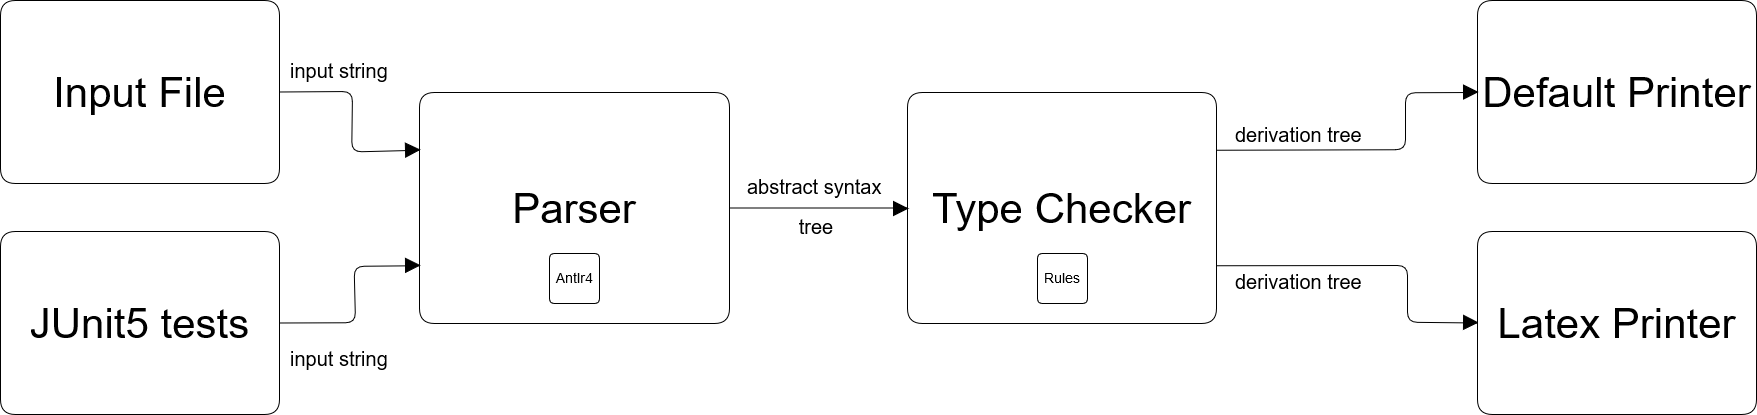
\includegraphics[scale=.25,keepaspectratio=true]{./typechecker.png}
 % gantt_chart.png: 0x0 pixel, 0dpi, nanxnan cm, bb=
 \caption{Project architecture.}
 \label{fig:gantt_chart}
\end{figure}

The project is implemented using Java and the executable is a jar file (target/TypeChecker.jar) which is generated using the command:
\definecolor{light-gray}{gray}{0.95}
\lstset{backgroundcolor= \color{light-gray}}

\begin{lstlisting}  
mvn install
\end{lstlisting}  

The program receives as an input a text file containing subtypes definitions and a judgment to be checked. For testing, \textbf{JUnit5} was used to test the program directly without files. The input is passed to the \textbf{Parser} which uses the ANTLR library to parse the input into an abstract syntax tree. This abstract syntax tree is consumed by the \textbf{Type Checker} which uses the rules in sections \ref{sec:simple} and \ref{sec:systemF} to build a derivation tree and determine the answer of the type checking. The answer can be \textbf{Yes}, \textbf{No}, or \textbf{Unknown}. Finally the derivation tree can be printed using the \textbf{Default Printer} or the \textbf{Latex Printer}.


Here is an example of an input:

\definecolor{light-gray}{gray}{0.95}

\lstset{caption={test.txt},backgroundcolor= \color{light-gray}}

\begin{lstlisting}  
SubBase(bool, int);
. |- \lambda x. \lambda y. (x y)[bool]: (int ->T) -> (bool -> T);
\end{lstlisting}

Here is the output of the default printer:

\lstset{caption={java -jar TypeChecker.jar -i test.txt}}

\begin{lstlisting}  
Yes
                                SubBase(bool, int)
-------------------(var)        -------------------(subBase)
x: bool ? x : bool                      bool <: int
--------------------------------------(subsumption)
x: bool ? x : int

\end{lstlisting}

Here is the output of the latex printer:

\lstset{caption={java -jar TypeChecker.jar -i test.txt -latex}}

\begin{lstlisting} 
Yes
\begin{prooftree}
\AxiomC{} \RightLabel{\scriptsize var}
\UnaryInfC{$x: bool \vdash x : bool$}
\AxiomC{\scriptsize $SubBase(bool,int)$}
\RightLabel{\scriptsize subBase}
\UnaryInfC{$bool <: int$}
\RightLabel{\scriptsize subsumption}
\BinaryInfC{$x: bool \vdash x : int$}
\end{prooftree}

\end{lstlisting} 

The following sections focus on terms and rules used in the \textbf{Type Checker}. 

\section{Simple types} \label{sec:simple}

Annotated simply typed terms recognized by the parser have the form:
\begin{align*}
t::= x \;|\; (t_1 t_2)[T]\;|\; \lambda x.t
\end{align*}

The annotation $[T]$ in the application term $(t_1 t_2)[T]$ is used to remove the non-determinism in the application rule. This annotation is required in the parser. 

\subsection{Typing rules for simple types} 

\begin{enumerate}

\item
\begin{prooftree}
\AxiomC{$\Gamma (x) = T$} \RightLabel{\scriptsize var} \UnaryInfC{$\Gamma \vdash x : T$}
\end{prooftree}
\item
\begin{prooftree}
\AxiomC{$\Gamma \vdash t_1 : T_1 \rightarrow T_2$} 
\AxiomC{$\Gamma \vdash t_2 : T_1$}
 \RightLabel{\scriptsize app} \BinaryInfC{$\Gamma \vdash (t_1 t_2)\color{blue}[T_1] \color{black} : T_2$}
\end{prooftree}
\item
\begin{prooftree}
\AxiomC{$\Gamma, x:T_1 \vdash t : T_2$} 
 \RightLabel{\scriptsize $\lambda$} \UnaryInfC{$\Gamma \vdash \lambda x .t:  T_1 \rightarrow T_2$}
\end{prooftree}

\end{enumerate}

\subsection{Subtyping rules for simple types} 

\begin{enumerate}

\item 

\begin{prooftree}
\AxiomC{$\Gamma \vdash t : T_1$} 
\AxiomC{$T_1 <: T_2$}
 \RightLabel{\scriptsize subsumption} \BinaryInfC{$\Gamma \vdash t: T_2$}
\end{prooftree}

\item 

\begin{prooftree}
\AxiomC{} 
 \RightLabel{\scriptsize reflexive} \UnaryInfC{$T <: T$}
\end{prooftree}
\item 

\begin{prooftree}
\AxiomC{$SubBase(b_1, b_2)$} 
 \RightLabel{\scriptsize subBase} \UnaryInfC{$b_1 <: b_2$}
\end{prooftree}
\item 

\begin{prooftree}
\AxiomC{$T'_1 <: T_1$} 
\AxiomC{$T_2 <: T'_2$}
 \RightLabel{\scriptsize arrow} \BinaryInfC{$T_1 \rightarrow T_2 <: T2_1 \rightarrow T'_2$}
\end{prooftree}

\item 

\begin{prooftree}
\AxiomC{$T_1 <: T_2$} 
\AxiomC{$T_2 <: T_3$}
 \RightLabel{\scriptsize transitive} \BinaryInfC{$T_1 <: T_3$}
\end{prooftree}


\end{enumerate}
\subsection{Examples}

Type checking is complete for annotated simply typed lambda calculus with subtypes. This means the answer is \textbf{Yes} if the judgment can be derived, and \textbf{No} if the judgment can not be derived. The Unknown answer is never returned because annotated simple types are decidable.

Here are some examples tested by the \textbf{TypeChecker}. A red rule in the derivation tree mean its judgment is not derivable. 


\begin{enumerate}



\item \textbf{Valid variable rule}

\begin{prooftree}
\AxiomC{} \RightLabel{\scriptsize var} \UnaryInfC{$x: T \vdash x : T$}
\end{prooftree}

\item \textbf{Invalid variable rule}

\begin{prooftree}
\AxiomC{} \RightLabel{\color{red} \scriptsize invalid var} \UnaryInfC{$\cdot \vdash x : T$} \color{black} 
\end{prooftree}

\item \textbf{Lambda \& application rules}

\begin{prooftree}
\AxiomC{} \RightLabel{var} \UnaryInfC{$x: (T1 \rightarrow T2), y: T1 \vdash x : (T1 \rightarrow T2)$}
\AxiomC{} \RightLabel{var} \UnaryInfC{$x: (T1 \rightarrow T2), y: T1 \vdash y : T1$}
\RightLabel{app} \BinaryInfC{$x: (T1 \rightarrow T2), y: T1 \vdash (x\;y) [T1] : T2$}
\RightLabel{$\lambda$}\UnaryInfC{$x: (T1 \rightarrow T2) \vdash  \lambda y. (x\;y) [T1] : (T1 \rightarrow T2)$}
\RightLabel{$\lambda$}\UnaryInfC{$\cdot \vdash  \lambda x.  \lambda y. (x\;y) [T1] : ((T1 \rightarrow T2) \rightarrow (T1 \rightarrow T2))$}
\end{prooftree}


\item \textbf{Direct Subtyping}

\begin{enumerate}

\item \textbf{Valid subtyping}
\begin{prooftree}
\AxiomC{} \RightLabel{\scriptsize var} \UnaryInfC{$x: bool \vdash x : bool$}
\AxiomC{\scriptsize SubBase($bool,int)$} \RightLabel{\scriptsize subBase} \UnaryInfC{$bool <: int$}
\RightLabel{\scriptsize subsumption} \BinaryInfC{$x: bool \vdash x : int$}
\end{prooftree}

\item \textbf{Invalid subtyping}

\begin{prooftree}
\AxiomC{} \RightLabel{\scriptsize var} \UnaryInfC{$x: int \vdash x : int$}
\AxiomC{\color{red} $\perp$ \color{black}} \RightLabel{\scriptsize \color{red} invalid \color{black}} \UnaryInfC{\color{red} $int <: bool$ \color{black}}
\RightLabel{\scriptsize subsumption} \BinaryInfC{$x: int \vdash x : bool$}
\end{prooftree}

\end{enumerate}

\item \textbf{Transitive subtyping}

\begin{prooftree}
\AxiomC{} \RightLabel{\scriptsize var} \UnaryInfC{$x: bool \vdash x : bool$}
\AxiomC{\scriptsize SubBase($bool,int)$} \RightLabel{\scriptsize subBase} \UnaryInfC{$bool <: int$}
\AxiomC{\scriptsize SubBase($int,double)$} \RightLabel{\scriptsize subBase} \UnaryInfC{$int <: double$}
\RightLabel{\scriptsize transitive} \BinaryInfC{$bool <: double$}
\RightLabel{\scriptsize subsumption} \BinaryInfC{$x: bool \vdash x : double$}
\end{prooftree}

\item  \textbf{Transitive subtyping}
\tiny
\begin{prooftree}
\AxiomC{} \RightLabel{\scriptsize var} \UnaryInfC{$x: bool \vdash x : bool$}
\AxiomC{\scriptsize SubBase($bool,int)$} \RightLabel{\scriptsize subBase} \UnaryInfC{$bool <: int$}
\AxiomC{\scriptsize SubBase($int,quotient)$} \RightLabel{\scriptsize subBase} \UnaryInfC{$int <: quotient$}
\RightLabel{\scriptsize transitive} \BinaryInfC{$bool <: quotient$}
\AxiomC{\scriptsize SubBase($quotient,double)$} \RightLabel{\scriptsize subBase} \UnaryInfC{$quotient <: double$}
\RightLabel{\scriptsize transitive} \BinaryInfC{$bool <: double$}
\RightLabel{\scriptsize subsumption} \BinaryInfC{$x: bool \vdash x : double$}
\end{prooftree}
\normalsize

\item \textbf{Arrow subtyping (subBase)}
\begin{prooftree}
\AxiomC{} \RightLabel{\scriptsize var} \UnaryInfC{$x: (int \rightarrow bool) \vdash x : (int \rightarrow bool)$}
\AxiomC{\scriptsize SubBase($bool,int)$} \RightLabel{\scriptsize subBase} \UnaryInfC{$bool <: int$}
\AxiomC{\scriptsize SubBase($bool,int)$} \RightLabel{\scriptsize subBase} \UnaryInfC{$bool <: int$}
\RightLabel{\scriptsize arrow} \BinaryInfC{$(int \rightarrow bool) <: (bool \rightarrow int)$}
\RightLabel{\scriptsize subsumption} \BinaryInfC{$x: (int \rightarrow bool) \vdash x : (bool \rightarrow int)$}
\end{prooftree}

\item \textbf{Arrow subtyping (reflexive, subBase)}
\begin{prooftree}
\AxiomC{} \RightLabel{\scriptsize var} \UnaryInfC{$x: (int \rightarrow bool) \vdash x : (int \rightarrow bool)$}
\AxiomC{} \RightLabel{\scriptsize reflexive} \UnaryInfC{$int <: int$}
\AxiomC{\scriptsize SubBase($bool,int)$} \RightLabel{\scriptsize subBase} \UnaryInfC{$bool <: int$}
\RightLabel{\scriptsize arrow} \BinaryInfC{$(int \rightarrow bool) <: (int \rightarrow int)$}
\RightLabel{\scriptsize subsumption} \BinaryInfC{$x: (int \rightarrow bool) \vdash x : (int \rightarrow int)$}
\end{prooftree}

\item \textbf{Arrow subtyping (reflexive, subBase)}

\tiny
\begin{prooftree}
\AxiomC{} \RightLabel{\scriptsize var} \UnaryInfC{$x: (int \rightarrow T), y: bool \vdash x : (int \rightarrow T)$}
\AxiomC{\scriptsize SubBase($bool,int)$} \RightLabel{\scriptsize subBase} \UnaryInfC{$bool <: int$}
\AxiomC{} \RightLabel{\scriptsize reflexive} \UnaryInfC{$T <: T$}
\RightLabel{\scriptsize arrow} \BinaryInfC{$(int \rightarrow T) <: (bool \rightarrow T)$}
\RightLabel{\scriptsize subsumption} \BinaryInfC{$x: (int \rightarrow T), y: bool \vdash x : (bool \rightarrow T)$}
\AxiomC{} \RightLabel{\scriptsize var} \UnaryInfC{$x: (int \rightarrow T), y: bool \vdash y : bool$}
\RightLabel{\scriptsize app} \BinaryInfC{$x: (int \rightarrow T), y: bool \vdash (x\;y) [bool] : T$}
\RightLabel{$\lambda$}\UnaryInfC{$x: (int \rightarrow T) \vdash  \lambda y. (x\;y) [bool] : (bool \rightarrow T)$}
\RightLabel{$\lambda$}\UnaryInfC{$\cdot \vdash  \lambda x.  \lambda y. (x\;y) [bool] : ((int \rightarrow T) \rightarrow (bool \rightarrow T))$}
\end{prooftree}

\normalsize

\item \textbf{Arrow subtyping (invalid)}

\begin{prooftree}
\AxiomC{} \RightLabel{\scriptsize var} \UnaryInfC{$x: (bool \rightarrow bool) \vdash x : (bool \rightarrow bool)$}
\AxiomC{\color{red} $\perp$ \color{black}} \RightLabel{\scriptsize \color{red} invalid \color{black}} \UnaryInfC{\color{red} $int <: bool$ \color{black}}
\AxiomC{\scriptsize SubBase($bool,int)$} \RightLabel{\scriptsize subBase} \UnaryInfC{$bool <: int$}
\RightLabel{\scriptsize arrow} \BinaryInfC{$(bool \rightarrow bool) <: (int \rightarrow int)$}
\RightLabel{\scriptsize subsumption} \BinaryInfC{$x: (bool \rightarrow bool) \vdash x : (int \rightarrow int)$}
\end{prooftree}

\item \textbf{Arrow subtyping (Invalid)}
\fontsize{4.2}{4}

\begin{prooftree}
\AxiomC{} \RightLabel{\tiny var} \UnaryInfC{$x: (bool \rightarrow T), y: bool \vdash x : (bool \rightarrow T)$}
\AxiomC{\color{red} $\perp$ \color{black}} \RightLabel{\tiny \color{red} invalid \color{black}} \UnaryInfC{\color{red} $int <: bool$ \color{black}}
\AxiomC{} \RightLabel{\tiny reflexive} \UnaryInfC{$T <: T$}
\RightLabel{\tiny arrow} \BinaryInfC{$(bool \rightarrow T) <: (int \rightarrow T)$}
\RightLabel{\tiny subsumption} \BinaryInfC{$x: (bool \rightarrow T), y: bool \vdash x : (int \rightarrow T)$}
\AxiomC{} \RightLabel{\tiny var} \UnaryInfC{$x: (bool \rightarrow T), y: bool \vdash y : bool$}
\AxiomC{\tiny SubBase($bool,int)$} \RightLabel{\tiny subBase} \UnaryInfC{$bool <: int$}
\RightLabel{\tiny subsumption} \BinaryInfC{$x: (bool \rightarrow T), y: bool \vdash y : int$}
\RightLabel{\tiny app} \BinaryInfC{$x: (bool \rightarrow T), y: bool \vdash (x\;y) [int] : T$}
\RightLabel{$\lambda$}\UnaryInfC{$x: (bool \rightarrow T) \vdash  \lambda y. (x\;y) [int] : (bool \rightarrow T)$}
\RightLabel{$\lambda$}\UnaryInfC{$\cdot \vdash  \lambda x.  \lambda y. (x\;y) [int] : ((bool \rightarrow T) \rightarrow (bool \rightarrow T))$}
\end{prooftree}

\normalsize

\end{enumerate}

\subsection{Delaying applying the subsumption rule}

The sumbumption rule can be delayed until the term in the judgment is a variable. This simplifies the code since there is only one rule to be applied for application and $\lambda$ abstraction terms. Here is the correctness proof using the subsumption rule: 

\begin{prooftree}
\AxiomC{$\Gamma \vdash t : T$} 
\AxiomC{$T <: T'$}
 \RightLabel{\scriptsize subsumption} \BinaryInfC{$\Gamma \vdash t: T'$}
\end{prooftree}


\begin{proof}

By induction hypothesis on the structure of the term $t$: 

\begin{enumerate}
\item Case $t=x$: trivial since $t$ is a variable. 

\begin{prooftree}
\AxiomC{$\Gamma \vdash x : T$} 
\AxiomC{$T <: T'$}
 \RightLabel{\scriptsize subsumption} \BinaryInfC{$\Gamma \vdash x: T'$}
\end{prooftree}

\item Case $t=t_1 t_2$: assume $T_2 <: T'_2$ and the following derivation:

\begin{prooftree}
\AxiomC{\color{blue} $\Gamma \vdash t_1 : T_1 \rightarrow T_2$ \color{black}} 
\AxiomC{\color{blue} $\Gamma \vdash t_2 : T_1$ \color{black}} 
\RightLabel{\scriptsize app}
\BinaryInfC{$\Gamma \vdash (t_1 t_2) [T_1] : T_2$} 
\AxiomC{\color{blue} $T_2 <: T'_2$ \color{black}}
\RightLabel{\scriptsize subsumption} 
\BinaryInfC{$\Gamma \vdash (t_1 t_2) [T_1]: T_2'$}
\end{prooftree}

We can get a different derivation tree where the sumbsumption rule is delayed:

\begin{prooftree}
\AxiomC{\color{blue} $\Gamma \vdash t_1 : T_1 \rightarrow T_2$ \color{black}} 
\AxiomC{} 
\RightLabel{\scriptsize reflexive}
\UnaryInfC{$T_1 <: T_1$} 
\AxiomC{\color{blue} $T_2 <: T'_2$ \color{black}}
\RightLabel{\scriptsize arrow}
\BinaryInfC{$T_1 \rightarrow T_2 <: T_1 \rightarrow T'_2$}
\RightLabel{\scriptsize subsumption}
\BinaryInfC{$\Gamma \vdash t_1 : T_1 \rightarrow T'_2$} 
\AxiomC{\color{blue} $\Gamma \vdash t_2 : T_1$ \color{black}} 
\RightLabel{\scriptsize app} 
\BinaryInfC{$\Gamma \vdash (t_1 t_2) [T_1]: T'_2$}
\end{prooftree}

Using the induction hypothesis, the subsumption rule can be delayed until variable terms are generated in the derivations of 
$\Gamma \vdash t_1 : T_1 \rightarrow T'_2$ and $\Gamma \vdash t_2 : T_1$.

\item Case $t=\lambda x. t'$: assume $T_1 \rightarrow T_2 <: T'_1 \rightarrow T'_2$ and the following derivation:

\begin{prooftree}
\AxiomC{\color{blue} $\Gamma, x:  T_1 \vdash t': T_2$ \color{black}} 
\RightLabel{\scriptsize $\lambda$}
\UnaryInfC{$\Gamma \vdash \lambda x. t': T_1 \rightarrow T_2$} 
\AxiomC{\color{blue} $T'_1 <: T_1$ \color{black}} 
\AxiomC{\color{blue} $T_2 <: T'_2$ \color{black}}
\RightLabel{\scriptsize arrow} 
\BinaryInfC{$T_1 \rightarrow T_2 <: T'_1 \rightarrow T'_2$}
\RightLabel{\scriptsize subsumption} 
\BinaryInfC{$\Gamma \vdash \lambda x. t': T'_1 \rightarrow T'_2$}
\end{prooftree}


Alternatively we can derive:

\begin{prooftree}
\AxiomC{\color{blue} $\Gamma, x: T'_1  \vdash t':  T_2$ \color{black}} 
\AxiomC{\color{blue} $T_2 <: T'_2$ \color{black}}
\RightLabel{\scriptsize subsumption} 
\BinaryInfC{$\Gamma, x: T'_1  \vdash t':  T'_2$} 
\RightLabel{\scriptsize $\lambda$} 
\UnaryInfC{$\Gamma \vdash \lambda x. t': T'_1 \rightarrow T'_2$}
\end{prooftree}

Assuming $T'_1 <: T_1$ is derivable, then by the subsumption rule:
\begin{prooftree}
\AxiomC{}
\RightLabel{\scriptsize var} 
\UnaryInfC{$\Gamma, x: T'_1 \vdash  x : T'_1 $}
\AxiomC{$T'_1 <: T_1$}
\RightLabel{\scriptsize subsumption} 
\BinaryInfC{$\Gamma, x: T'_1 \vdash  x : T_1 $}
\end{prooftree}

Therefore if $\Gamma, x: T_1  \vdash t':  T_2$ is derivable, then $\Gamma, x: T'_1  \vdash t':  T_2$ is also derivable which concludes the proof. 

\end{enumerate}

\end{proof}

\begin{remark} 

If $\Gamma, x: T'_1  \vdash t':  T_2$, it is not always true  that $\Gamma, x: T_1  \vdash t':  T_2$ where $T'_1 <: T_1$.

\end{remark}

 A counter example would be 
\begin{align*}
x: bool \vdash x: int \nRightarrow x:double \vdash x: int,\;\;\; bool <: int <: double
\end{align*}
However 
\begin{align*}
x: int \vdash x: double \Rightarrow x:bool \vdash x: double,\;\;\; bool <: int <: double
\end{align*}

Therefore in the following example, using the subsumption rule first would fail and slow the type checker because it needs to backtrack and check the $\lambda$ rule. However using the $\lambda$ rule first would prove the derivation and it is faster. 


\begin{prooftree}
\AxiomC{\color{red} $\ x:  double \vdash x: int$ \color{black}} 
\RightLabel{\scriptsize $\lambda$}
\UnaryInfC{$\Gamma \vdash \lambda x. x: double \rightarrow int$} 
\AxiomC{$SubBase(bool, double)$}
\RightLabel{\scriptsize subBase} 
\UnaryInfC{$bool <: double$} 
\AxiomC{}
\RightLabel{\scriptsize reflexive} 
\UnaryInfC{$int <: int$}
\RightLabel{\scriptsize arrow} 
\BinaryInfC{$double \rightarrow int <: bool \rightarrow int$}
\RightLabel{\scriptsize subsumption} 
\BinaryInfC{$\Gamma \vdash \lambda x. x: bool \rightarrow int$}
\end{prooftree}



\begin{prooftree}
\AxiomC{} 
\RightLabel{\scriptsize var} 
\UnaryInfC{$\Gamma, x: bool \vdash x:  bool$} 
\AxiomC{$SubBase(bool, int)$} 
\RightLabel{\scriptsize suBase} 
\UnaryInfC{$bool <: int$}
\RightLabel{\scriptsize subsumption} 
\BinaryInfC{$\Gamma, x: bool  \vdash x:  int$} 
\RightLabel{\scriptsize $\lambda$} 
\UnaryInfC{$\Gamma \vdash \lambda x. x: bool \rightarrow int$}
\end{prooftree}




\section{System F} \label{sec:systemF}

Annotated system F terms, and types recognized by the parser have the form:
\begin{align*}
t &::= x \;|\; (t_1 t_2)[T]\;|\; \lambda x.t\; | \; t\; [[T]] \\
T &::= X \; | T_1 \rightarrow T_2 \; | \; \forall X. T
\end{align*}

The annotation $[T]$ in the application term $(t_1 t_2)[T]$ is used to remove the non-determinism in the application rule. The annotation $[[T]]$ in the term $t [[T]]$ is used to remove the non-determinism in the elimination rule. Unlike the application annotation, the elimination annotation is not required in the parser which makes the \textbf{TypeChecker} incomplete. Whenever the \textbf{TypeChecker} needs the elimination annotation and it is not provided, it returns the current derivation tree with answer \textbf{Unknown}. 

\subsection{Rules}

\begin{enumerate}

\item If $X$ is not free in $\Gamma$

\begin{prooftree}
\AxiomC{$\Gamma \vdash t: T$} 
\RightLabel{\scriptsize introduction} 
\UnaryInfC{$\Gamma \vdash t: \forall X.T$}
\end{prooftree}

\item If $X$ is free in $\Gamma$, choose $X_i$ such that $X_i$ is not free in $\Gamma$

\begin{prooftree}
\AxiomC{$\Gamma \vdash t: [X_i/X]T$} 
\RightLabel{\scriptsize introduction} 
\UnaryInfC{$\Gamma \vdash t: \forall X_i.[X_i/X]T$} 
\RightLabel{\scriptsize renaming} 
\UnaryInfC{$\Gamma \vdash t: \forall X.T$}
\end{prooftree}

\item Elimination rule with annotation

\begin{prooftree}
\AxiomC{$\Gamma \vdash t: \forall X. [X/T']T$} 
\RightLabel{\scriptsize elimination} 
\UnaryInfC{$\Gamma \vdash t\;[[T']]: T$}
\end{prooftree}

\end{enumerate}

\subsection{Examples}

Here are some examples tested by the \textbf{TypeChecker}. A red rule in the derivation tree mean its judgment is not derivable. A blue rule means the \textbf{TypeChecker} needs more annotation to continue the type checking. 

\begin{enumerate}


\item Same type variable

\begin{prooftree}
\AxiomC{} \RightLabel{\scriptsize var} \UnaryInfC{$x: \forall X.X \vdash x : \forall X.X$}
\end{prooftree}

\item Different type variables

\begin{prooftree}
\AxiomC{} \RightLabel{\scriptsize var} \UnaryInfC{$x: \forall X.X \vdash x : \forall Y.Y$}
\end{prooftree}

\item Arrows
\begin{prooftree}
\AxiomC{} \RightLabel{\scriptsize var} \UnaryInfC{$x: \forall X.(X \rightarrow X) \vdash x : \forall Y.(Y \rightarrow Y)$}
\end{prooftree}

\item $Y$ is free in the typing context and the term type

\begin{prooftree}
\AxiomC{} \RightLabel{\scriptsize var} \UnaryInfC{$x: \forall X.(X \rightarrow Y) \vdash x : \forall Z.(Z \rightarrow Y)$}
\end{prooftree}

\item $Y$ is free in the typing context
\begin{prooftree}
\AxiomC{} \RightLabel{\color{red} \scriptsize invalid var} \UnaryInfC{$x: \forall X.(X \rightarrow Y) \vdash x : \forall Y.(Y \rightarrow Y)$} \color{black} 
\end{prooftree}

\item $Y$ is free in the typing context, and $Z$ is free in the term type

\begin{prooftree}
\AxiomC{} \RightLabel{\color{red} \scriptsize invalid var} \UnaryInfC{$x: \forall X.(X \rightarrow Y) \vdash x : \forall Y.(Y \rightarrow Z)$} \color{black} 
\end{prooftree}

\item Elimination annotation

\begin{prooftree}
\AxiomC{} \RightLabel{\scriptsize var} \UnaryInfC{$x: \forall X.X \vdash x : \forall X1.X1$}
\RightLabel{\scriptsize elimination}\UnaryInfC{$x: \forall X.X \vdash x[Y] : Y$}
\end{prooftree}

\item Elimination annotation with arrow
\begin{prooftree}
\AxiomC{} \RightLabel{\scriptsize var} \UnaryInfC{$x: \forall X.X \vdash x : \forall X1.X1$}
\RightLabel{\scriptsize elimination}\UnaryInfC{$x: \forall X.X \vdash x[(Y \rightarrow Y)] : (Y \rightarrow Y)$}
\end{prooftree}

\item Nested elimination annotation
\tiny
\begin{prooftree}
\AxiomC{} \RightLabel{\scriptsize var} \UnaryInfC{$x: \forall X.X \vdash x : \forall X1.X1$}
\RightLabel{\scriptsize elimination}\UnaryInfC{$x: \forall X.X \vdash x[[(\forall X.X \rightarrow \forall X.X)]][(\forall X.X \rightarrow \forall X.X)] : (\forall X.X \rightarrow \forall X.X)$}
\AxiomC{} \RightLabel{\scriptsize var} \UnaryInfC{$x: \forall X.X \vdash x : \forall X.X$}
\RightLabel{\scriptsize app} \BinaryInfC{$x: \forall X.X \vdash (x[[(\forall X.X \rightarrow \forall X.X)]]\;x) [\forall X.X] : \forall X.X$}
\end{prooftree}

\normalsize

\item Application or introduction non-determinism: The \textbf{TypeChecker} attempts applications first. When it fails, it backtracks and attempts the introduction rule as shown in the next example. 
\tiny
\begin{prooftree}
\AxiomC{} \RightLabel{\scriptsize var}
\UnaryInfC{$x: (T_1 \rightarrow T_2), y: T_1 \vdash x : (T_1 \rightarrow T_2)$}
\AxiomC{} \RightLabel{\scriptsize reflexive}
 \UnaryInfC{$T_1 <: T_1$}
\AxiomC{\color{red} $\perp$ \color{black}} 
\RightLabel{\scriptsize \color{red} invalid \color{black}}
\UnaryInfC{\color{red} $T_2 <: \forall X.T_2$ \color{black}}
\RightLabel{\scriptsize arrow}
\BinaryInfC{$(T_1 \rightarrow T_2) <: (T_1 \rightarrow \forall X.T_2)$}
\RightLabel{\scriptsize subsumption}
\BinaryInfC{$x: (T_1 \rightarrow T_2), y: T_1 \vdash x : (T_1 \rightarrow \forall X.T_2)$}
\AxiomC{} \RightLabel{\scriptsize var}
\UnaryInfC{$x: (T_1 \rightarrow T_2), y: T_1 \vdash y : T_1$}
\RightLabel{\scriptsize app}
\BinaryInfC{$x: (T_1 \rightarrow T_2), y: T_1 \vdash (x\;y) [T_1] : \forall X.T_2$}
\end{prooftree}

\normalsize
\item Introduction branch
\begin{prooftree}
\AxiomC{} \RightLabel{\scriptsize var}
\UnaryInfC{$x: (T_1 \rightarrow T_2), y: T_1 \vdash x : (T_1 \rightarrow T_2)$}
\AxiomC{} \RightLabel{\scriptsize var}
\UnaryInfC{$x: (T_1 \rightarrow T_2), y: T_1 \vdash y : T_1$}
\RightLabel{\scriptsize app}
\BinaryInfC{$x: (T_1 \rightarrow T_2), y: T_1 \vdash (x\;y) [T_1] : T_2$}
\RightLabel{\scriptsize introduction}
\UnaryInfC{$x: (T_1 \rightarrow T_2), y: T_1 \vdash (x\;y) [T_1] : \forall X.T_2$}
\end{prooftree}


\item Application or elimination non-determinism 
\tiny

\begin{prooftree}
\AxiomC{} \RightLabel{\scriptsize var}
\UnaryInfC{$x: (T_1 \rightarrow \forall X.T_2), y: T_1 \vdash x : (T_1 \rightarrow \forall X.T_2)$}
\AxiomC{} \RightLabel{\scriptsize reflexive}
 \UnaryInfC{$T_1 <: T_1$}
\AxiomC{\color{red} $\perp$ \color{black}} 
\RightLabel{\scriptsize \color{red} invalid \color{black}}
\UnaryInfC{\color{red} $\forall X.T_2 <: T_2$ \color{black}}
\RightLabel{\scriptsize arrow}
\BinaryInfC{$(T_1 \rightarrow \forall X.T_2) <: (T_1 \rightarrow T_2)$}
\RightLabel{\scriptsize subsumption}
\BinaryInfC{$x: (T_1 \rightarrow \forall X.T_2), y: T_1 \vdash x : (T_1 \rightarrow T_2)$}
\AxiomC{} \RightLabel{\scriptsize var}
\UnaryInfC{$x: (T_1 \rightarrow \forall X.T_2), y: T_1 \vdash y : T_1$}
\RightLabel{\scriptsize app}
\BinaryInfC{$x: (T_1 \rightarrow \forall X.T_2), y: T_1 \vdash (x\;y) [T_1][[Y]] : T_2$}
\end{prooftree}

\normalsize

\item Elimination branch

\begin{prooftree}
\AxiomC{} \RightLabel{\scriptsize var}
\UnaryInfC{$x: (T_1 \rightarrow \forall X.T_2), y: T_1 \vdash x : (T_1 \rightarrow \forall X_1.T_2)$}
\AxiomC{} \RightLabel{\scriptsize var}
\UnaryInfC{$x: (T_1 \rightarrow \forall X.T_2), y: T_1 \vdash y : T_1$}
\RightLabel{\scriptsize app}
\BinaryInfC{$x: (T_1 \rightarrow \forall X.T_2), y: T_1 \vdash (x\;y) [T_1] : \forall X_1.T_2$}
\RightLabel{\scriptsize elimination}
\UnaryInfC{$x: (T_1 \rightarrow \forall X.T_2), y: T_1 \vdash (x\;y) [T_1][[Y]] : T_2$}
\end{prooftree}

\normalsize

\item Zero

\begin{prooftree}
\AxiomC{} \RightLabel{\scriptsize var} \UnaryInfC{$z: X, s: (X \rightarrow X) \vdash z : X$}
\RightLabel{$\lambda$}\UnaryInfC{$s: (X \rightarrow X) \vdash (\lambda z. z) : (X \rightarrow X)$}
\RightLabel{$\lambda$}\UnaryInfC{$\cdot \vdash (\lambda s. (\lambda z. z)) : ((X \rightarrow X) \rightarrow (X \rightarrow X))$}
\RightLabel{\scriptsize introduction}\UnaryInfC{$\cdot \vdash (\lambda s. (\lambda z. z)) : \forall X.((X \rightarrow X) \rightarrow (X \rightarrow X))$}
\end{prooftree}

\item Zero with free variable $X$

\begin{prooftree}
\AxiomC{} \RightLabel{\scriptsize var}
\UnaryInfC{$y: X, z: X_2, s: (X_2 \rightarrow X_2) \vdash z : X_2$}
\RightLabel{$\lambda$}
\UnaryInfC{$y: X, s: (X_2 \rightarrow X_2) \vdash (\lambda z. z) : (X_2 \rightarrow X_2)$}
\RightLabel{$\lambda$}
\UnaryInfC{$y: X \vdash (\lambda s. (\lambda z. z)) : ((X_2 \rightarrow X_2) \rightarrow (X_2 \rightarrow X_2))$}
\RightLabel{\scriptsize introduction}
\UnaryInfC{$y: X \vdash (\lambda s. (\lambda z. z)) : \forall X_2.((X_2 \rightarrow X_2) \rightarrow (X_2 \rightarrow X_2))$}
\RightLabel{\scriptsize renaming}
\UnaryInfC{$y: X \vdash (\lambda s. (\lambda z. z)) : \forall X.((X \rightarrow X) \rightarrow (X \rightarrow X))$}
\end{prooftree}

\end{enumerate}

\begin{landscape}

Successor missing annotation
\fontsize{3}{4}
\begin{prooftree}
\AxiomC{} \RightLabel{\tiny var}
\UnaryInfC{$n: \forall X.((X \rightarrow X) \rightarrow (X \rightarrow X)), z: X, s: (X \rightarrow X) \vdash s : (X \rightarrow X)$}
\AxiomC{}
\RightLabel{\color{blue} \tiny unknown}
\UnaryInfC{$n: \forall X.((X \rightarrow X) \rightarrow (X \rightarrow X)), z: X, s: (X \rightarrow X) \vdash n : ((X \rightarrow X) \rightarrow (X \rightarrow X))$ \color{black}}  
\AxiomC{} \RightLabel{\tiny var}
\UnaryInfC{$n: \forall X.((X \rightarrow X) \rightarrow (X \rightarrow X)), z: X, s: (X \rightarrow X) \vdash s : (X \rightarrow X)$}
\RightLabel{\tiny app}
\BinaryInfC{$n: \forall X.((X \rightarrow X) \rightarrow (X \rightarrow X)), z: X, s: (X \rightarrow X) \vdash (n\;s) [(X \rightarrow X)] : (X \rightarrow X)$}
\AxiomC{} \RightLabel{\tiny var}
\UnaryInfC{$n: \forall X.((X \rightarrow X) \rightarrow (X \rightarrow X)), z: X, s: (X \rightarrow X) \vdash z : X$}
\RightLabel{\tiny app}
\BinaryInfC{$n: \forall X.((X \rightarrow X) \rightarrow (X \rightarrow X)), z: X, s: (X \rightarrow X) \vdash ((n\;s) [(X \rightarrow X)]\;z) [X] : X$}
\RightLabel{\tiny app}
\BinaryInfC{$n: \forall X.((X \rightarrow X) \rightarrow (X \rightarrow X)), z: X, s: (X \rightarrow X) \vdash (s\;((n\;s) [(X \rightarrow X)]\;z) [X]) [X] : X$}
\RightLabel{$\lambda$}
\UnaryInfC{$n: \forall X.((X \rightarrow X) \rightarrow (X \rightarrow X)), s: (X \rightarrow X) \vdash (\lambda z. (s\;((n\;s) [(X \rightarrow X)]\;z) [X]) [X]) : (X \rightarrow X)$}
\RightLabel{$\lambda$}
\UnaryInfC{$n: \forall X.((X \rightarrow X) \rightarrow (X \rightarrow X)) \vdash (\lambda s. (\lambda z. (s\;((n\;s) [(X \rightarrow X)]\;z) [X]) [X])) : ((X \rightarrow X) \rightarrow (X \rightarrow X))$}
\RightLabel{\tiny introduction}
\UnaryInfC{$n: \forall X.((X \rightarrow X) \rightarrow (X \rightarrow X)) \vdash (\lambda s. (\lambda z. (s\;((n\;s) [(X \rightarrow X)]\;z) [X]) [X])) : \forall X.((X \rightarrow X) \rightarrow (X \rightarrow X))$}
\RightLabel{$\lambda$}
\UnaryInfC{$\cdot \vdash (\lambda n. (\lambda s. (\lambda z. (s\;((n\;s) [(X \rightarrow X)]\;z) [X]) [X]))) : (\forall X.((X \rightarrow X) \rightarrow (X \rightarrow X)) \rightarrow \forall X.((X \rightarrow X) \rightarrow (X \rightarrow X)))$}
\end{prooftree}

\normalsize
Successor well annotated

\fontsize{3}{4}

\begin{prooftree}
\AxiomC{} \RightLabel{\tiny var}
\UnaryInfC{$n: \forall X.((X \rightarrow X) \rightarrow (X \rightarrow X)), z: X, s: (X \rightarrow X) \vdash s : (X \rightarrow X)$}
\AxiomC{} \RightLabel{\tiny var}
\UnaryInfC{$n: \forall X.((X \rightarrow X) \rightarrow (X \rightarrow X)), z: X, s: (X \rightarrow X) \vdash n : \forall X1.((X1 \rightarrow X1) \rightarrow (X1 \rightarrow X1))$}
\RightLabel{\tiny elimination}
\UnaryInfC{$n: \forall X.((X \rightarrow X) \rightarrow (X \rightarrow X)), z: X, s: (X \rightarrow X) \vdash n[[X]][X] : ((X \rightarrow X) \rightarrow (X \rightarrow X))$}
\AxiomC{} \RightLabel{\tiny var}
\UnaryInfC{$n: \forall X.((X \rightarrow X) \rightarrow (X \rightarrow X)), z: X, s: (X \rightarrow X) \vdash s : (X \rightarrow X)$}
\RightLabel{\tiny app}
\BinaryInfC{$n: \forall X.((X \rightarrow X) \rightarrow (X \rightarrow X)), z: X, s: (X \rightarrow X) \vdash (n[[X]]\;s) [(X \rightarrow X)] : (X \rightarrow X)$}
\AxiomC{} \RightLabel{\tiny var}
\UnaryInfC{$n: \forall X.((X \rightarrow X) \rightarrow (X \rightarrow X)), z: X, s: (X \rightarrow X) \vdash z : X$}
\RightLabel{\tiny app}
\BinaryInfC{$n: \forall X.((X \rightarrow X) \rightarrow (X \rightarrow X)), z: X, s: (X \rightarrow X) \vdash ((n[[X]]\;s) [(X \rightarrow X)]\;z) [X] : X$}
\RightLabel{\tiny app}
\BinaryInfC{$n: \forall X.((X \rightarrow X) \rightarrow (X \rightarrow X)), z: X, s: (X \rightarrow X) \vdash (s\;((n[[X]]\;s) [(X \rightarrow X)]\;z) [X]) [X] : X$}
\RightLabel{$\lambda$}
\UnaryInfC{$n: \forall X.((X \rightarrow X) \rightarrow (X \rightarrow X)), s: (X \rightarrow X) \vdash (\lambda z. (s\;((n[[X]]\;s) [(X \rightarrow X)]\;z) [X]) [X]) : (X \rightarrow X)$}
\RightLabel{$\lambda$}
\UnaryInfC{$n: \forall X.((X \rightarrow X) \rightarrow (X \rightarrow X)) \vdash (\lambda s. (\lambda z. (s\;((n[[X]]\;s) [(X \rightarrow X)]\;z) [X]) [X])) : ((X \rightarrow X) \rightarrow (X \rightarrow X))$}
\RightLabel{\tiny introduction}
\UnaryInfC{$n: \forall X.((X \rightarrow X) \rightarrow (X \rightarrow X)) \vdash (\lambda s. (\lambda z. (s\;((n[[X]]\;s) [(X \rightarrow X)]\;z) [X]) [X])) : \forall X.((X \rightarrow X) \rightarrow (X \rightarrow X))$}
\RightLabel{$\lambda$}
\UnaryInfC{$\cdot \vdash (\lambda n. (\lambda s. (\lambda z. (s\;((n[[X]]\;s) [(X \rightarrow X)]\;z) [X]) [X]))) : (\forall X.((X \rightarrow X) \rightarrow (X \rightarrow X)) \rightarrow \forall X.((X \rightarrow X) \rightarrow (X \rightarrow X)))$}
\end{prooftree}

\end{landscape}

\end{document}
